

%\begin{frame}{Need}
%\textbf{Congestion Control} = Crucial part of \textbf{App Performance}
%\end{frame}


\begin{frame}{Motivation}
\begin{itemize}
\item NFD congestion detection doesn't work in ndnSIM\\ (no real TCP/UDP/Unix faces)
\pause
\item Tasks: Fix that. 
%\begin{itemize}
%\item Implement a ns-3 Queue based on CoDel that detects congestion and inserts congestion marks.
%\item Map these congestion marks onto NDNLP/ns-3 packets.
%\end{itemize}
%\item Additional Tasks (if time):
%\begin{itemize}
%\item Start submitting the code to Gerrit.
%\item Implement a TCP-Cubic like consumer app and compare it against the AIMD app.
%\end{itemize}
\end{itemize}
\end{frame}



\begin{frame}{Solution Steps}

\begin{enumerate}
\item \textbf{ndnSIM doesn't use real TCP or UDP faces.}\\
$\Rightarrow$ NetDeviceTransport: override
virtual function(s) for congestion control.
\pause

\item \textbf{CongestionMarks sent over NDNLP:} Already works! 
\pause

\item \textbf{Implement Consumer App} that reacts to congestion marks (AIMD and TCP CUBIC)

\end{enumerate}

\end{frame}


\begin{frame}{Evaluation Scenario}

Very simple scenario: 

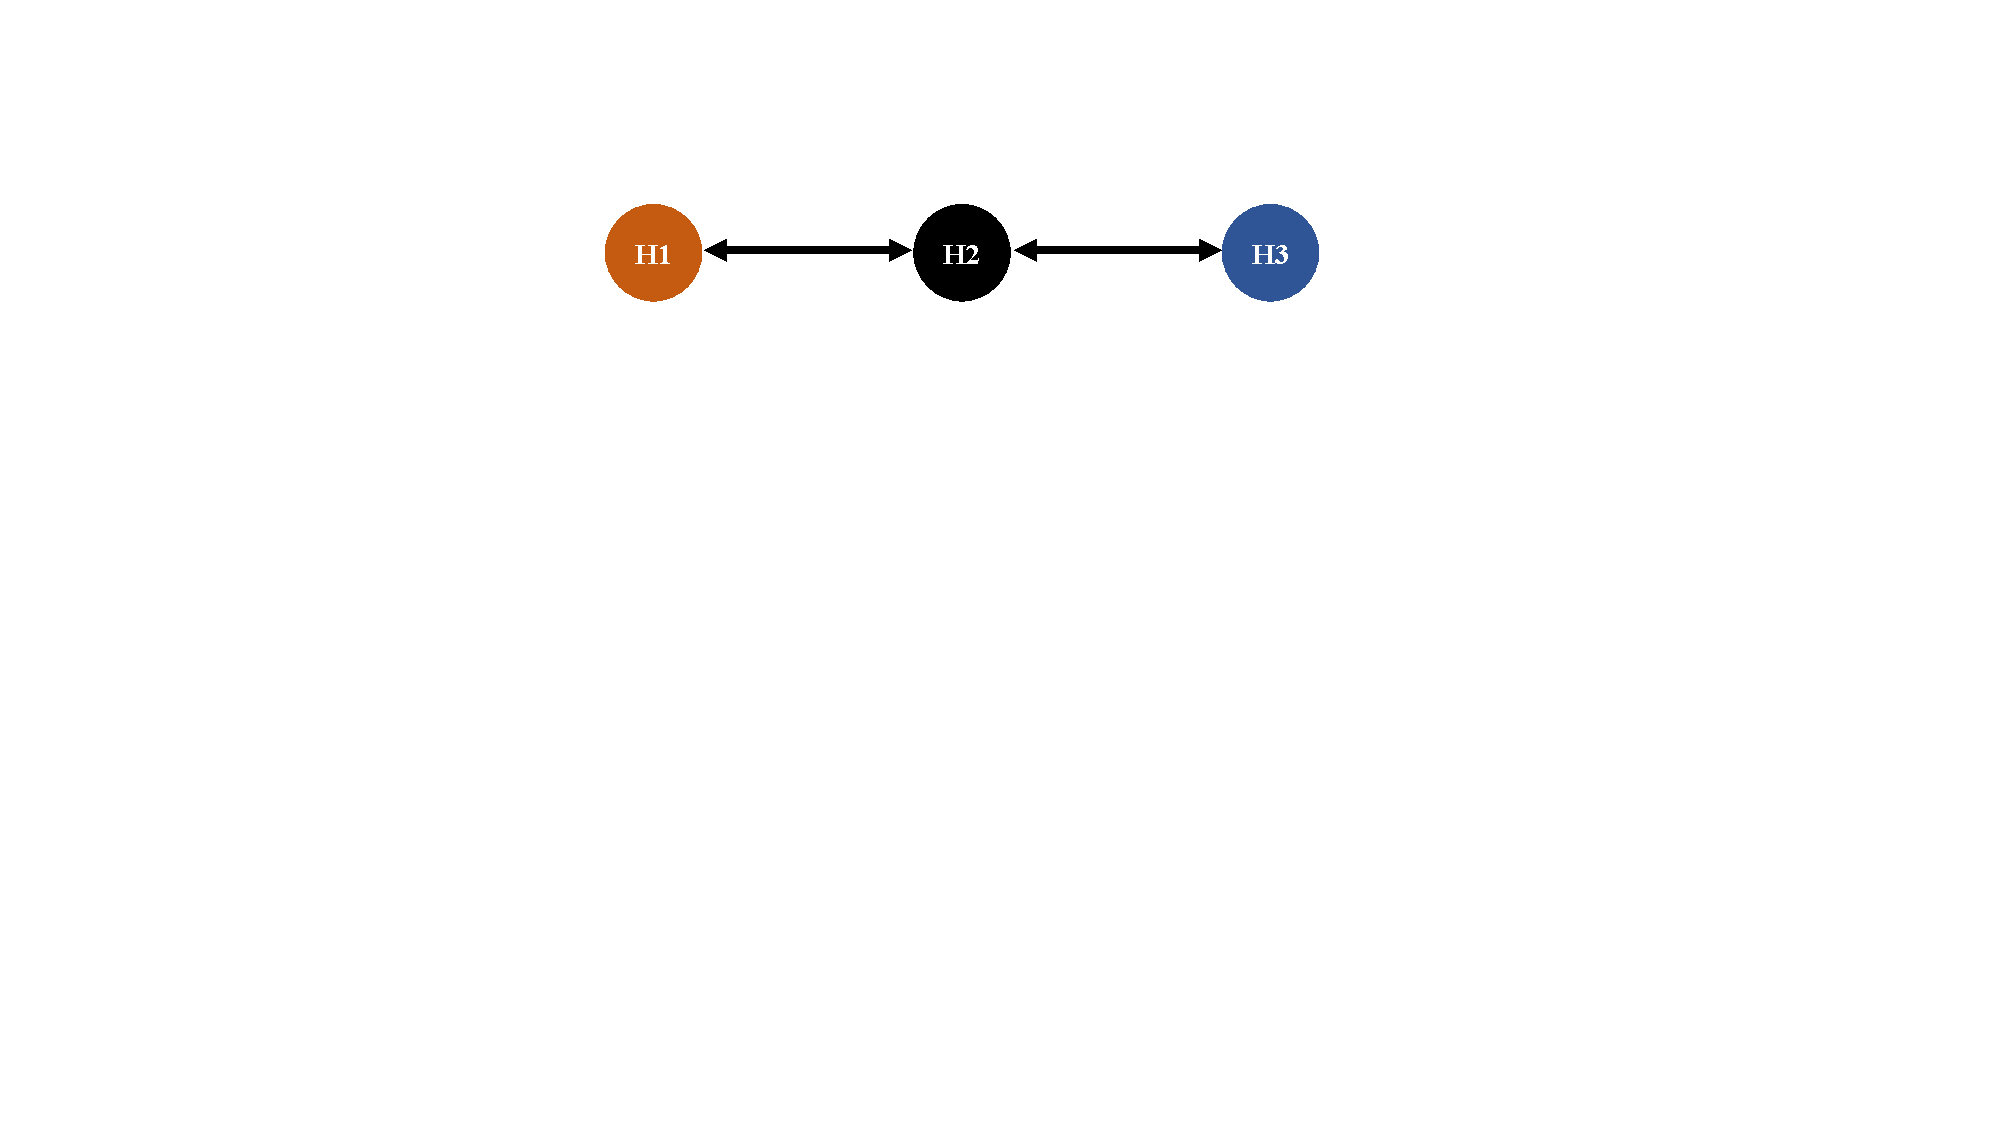
\includegraphics[width=\linewidth]{figs/Figure_3.pdf}

\begin{itemize}
\item 1 Consumer, Runtime: 40s 
%\item 
\item RTT: 40ms 
\item Bottleneck capacity: 50 Mbit/s 
\end{itemize}


\end{frame}


\begin{frame}{How ndnSIM performs right now}

ConsumerWindow App: 

\begin{itemize}
\item On Data: $m_{cwnd}$++ (constant slow start!)
\item On Timeout: $m_{cwnd} \leftarrow 2$
\end{itemize}

\pause
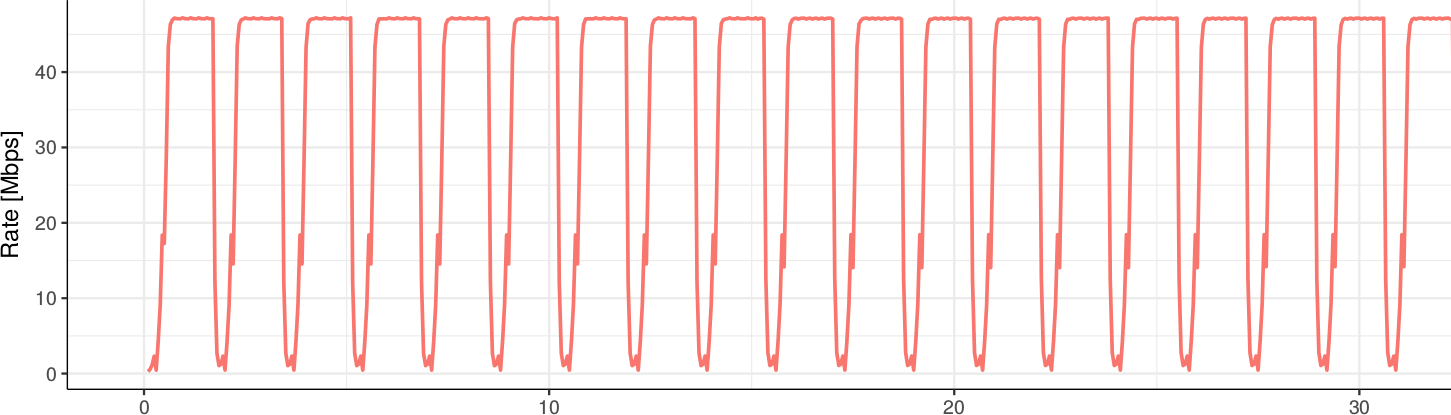
\includegraphics[width=\linewidth]{figs/cons1.png}


\end{frame}

\begin{frame}{How ndnSIM performs right now}

60,000 Timeouts!!!

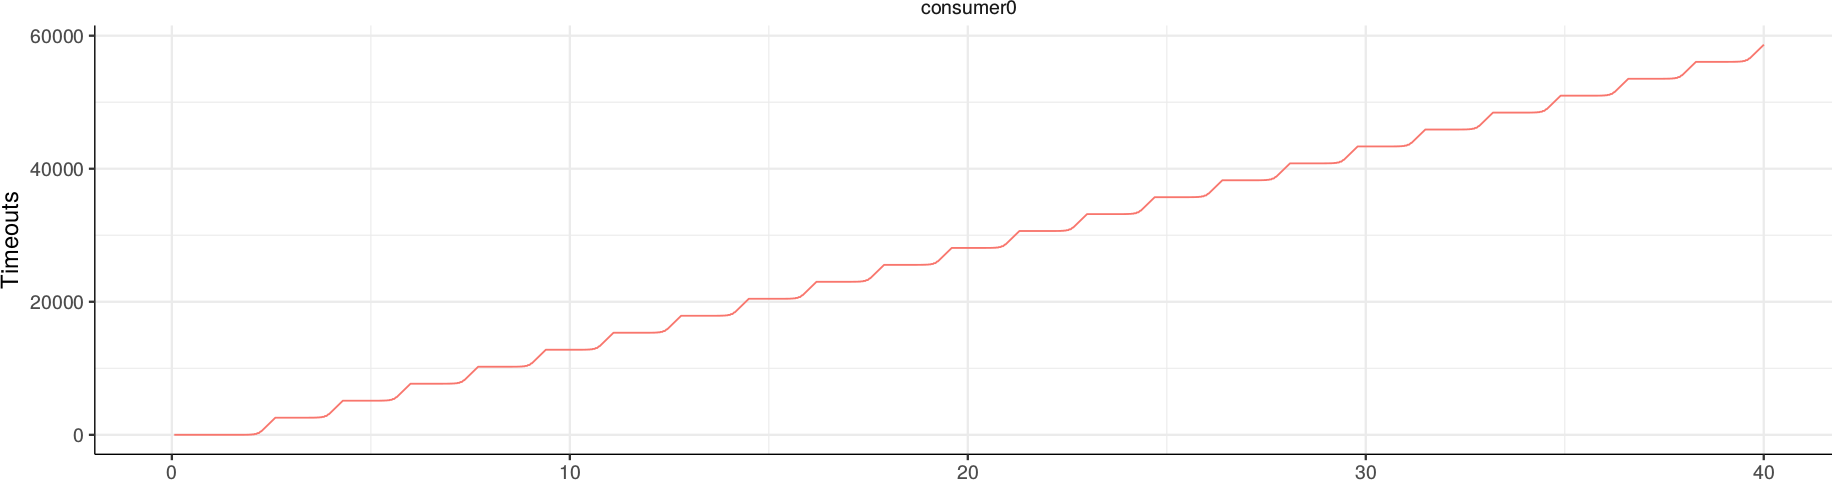
\includegraphics[width=\linewidth]{figs/cons2.png}


\end{frame}


\begin{frame}{Improved ConsumerWindow (no congestion marks)}

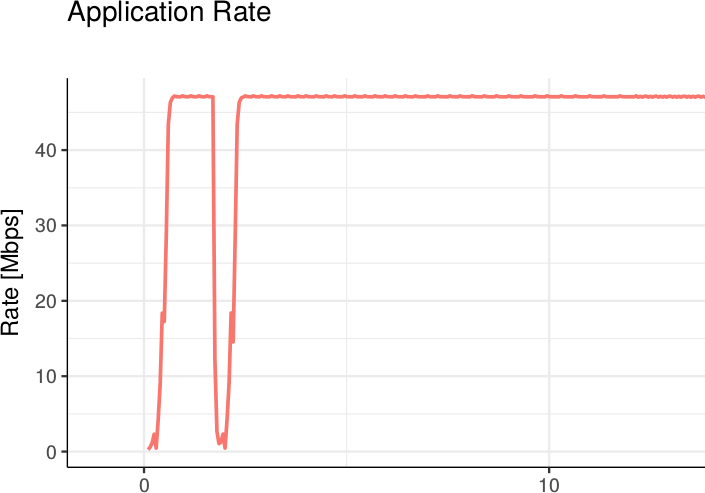
\includegraphics[width=0.48\linewidth]{figs/cons_new_rate.png}
\hspace{.1em}
\pause
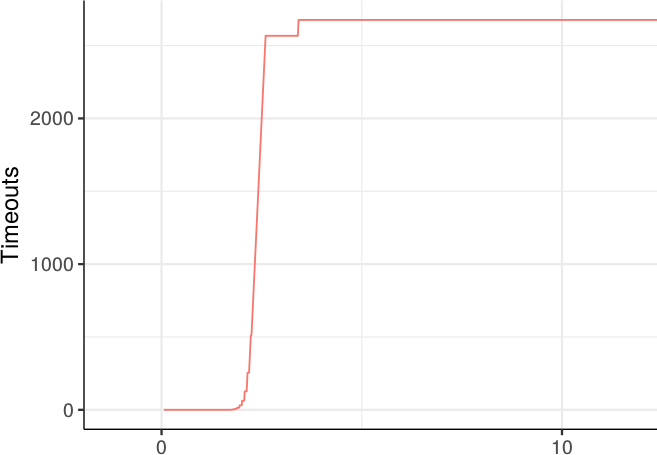
\includegraphics[width=0.48\linewidth]{figs/cons_new_timeouts.png}\\
\pause
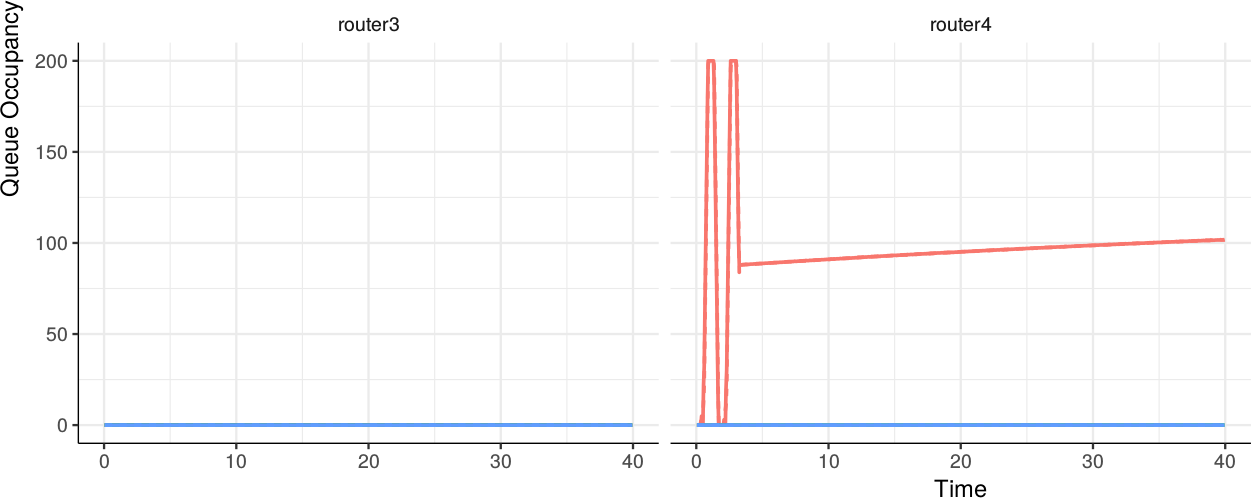
\includegraphics[width=\linewidth]{figs/cons_new_queue.png}

\end{frame}


\begin{frame}{ConsumerPCON -- AIMD}

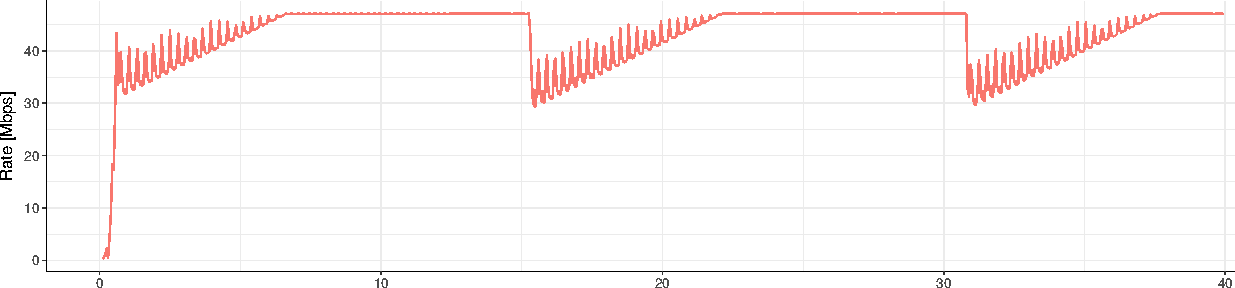
\includegraphics[width=\linewidth]{figs/cons_pcon_rate.png}\\
\only<1-2>{
No Timeouts!, Shorter ``sawtooth'' patterns (about 15s)
}
\pause
\includegraphics<1-2>[width=\linewidth]{figs/cons_pcon_queue.png}

\end{frame}


\begin{frame}{ConsumerPCON -- CUBIC}

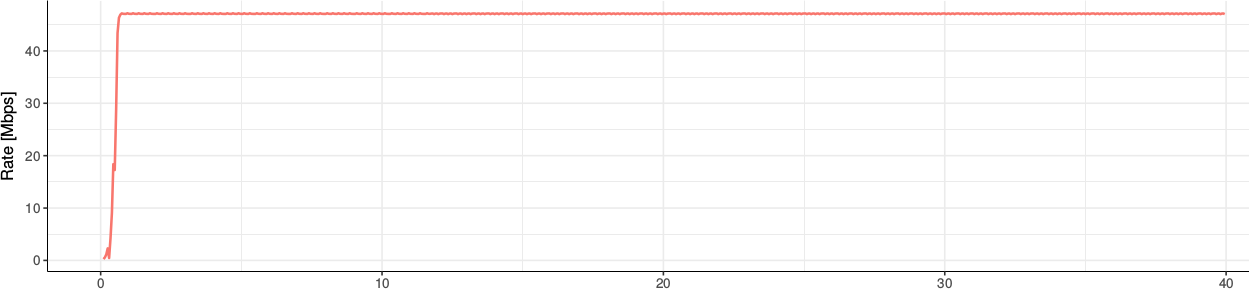
\includegraphics[width=\linewidth]{figs/cons_cubic_rate.png}\\
\pause
\includegraphics<1-2>[width=\linewidth]{figs/cons_cubic_queue.png}

Even Shorter Sawtooths (about 7s)!

\end{frame}


\begin{frame}{Future Work}

Congestion Detection via adapted CoDelQueue:
\begin{itemize}
\item Worked well in ns3 3.23 (PCON simulation code)
\pause
\item Doesn't work anymore in ns3 3.27 (current ndnSIM)
\end{itemize}

\pause
NS-3 separated queuing in traffic-control module as:

\centering
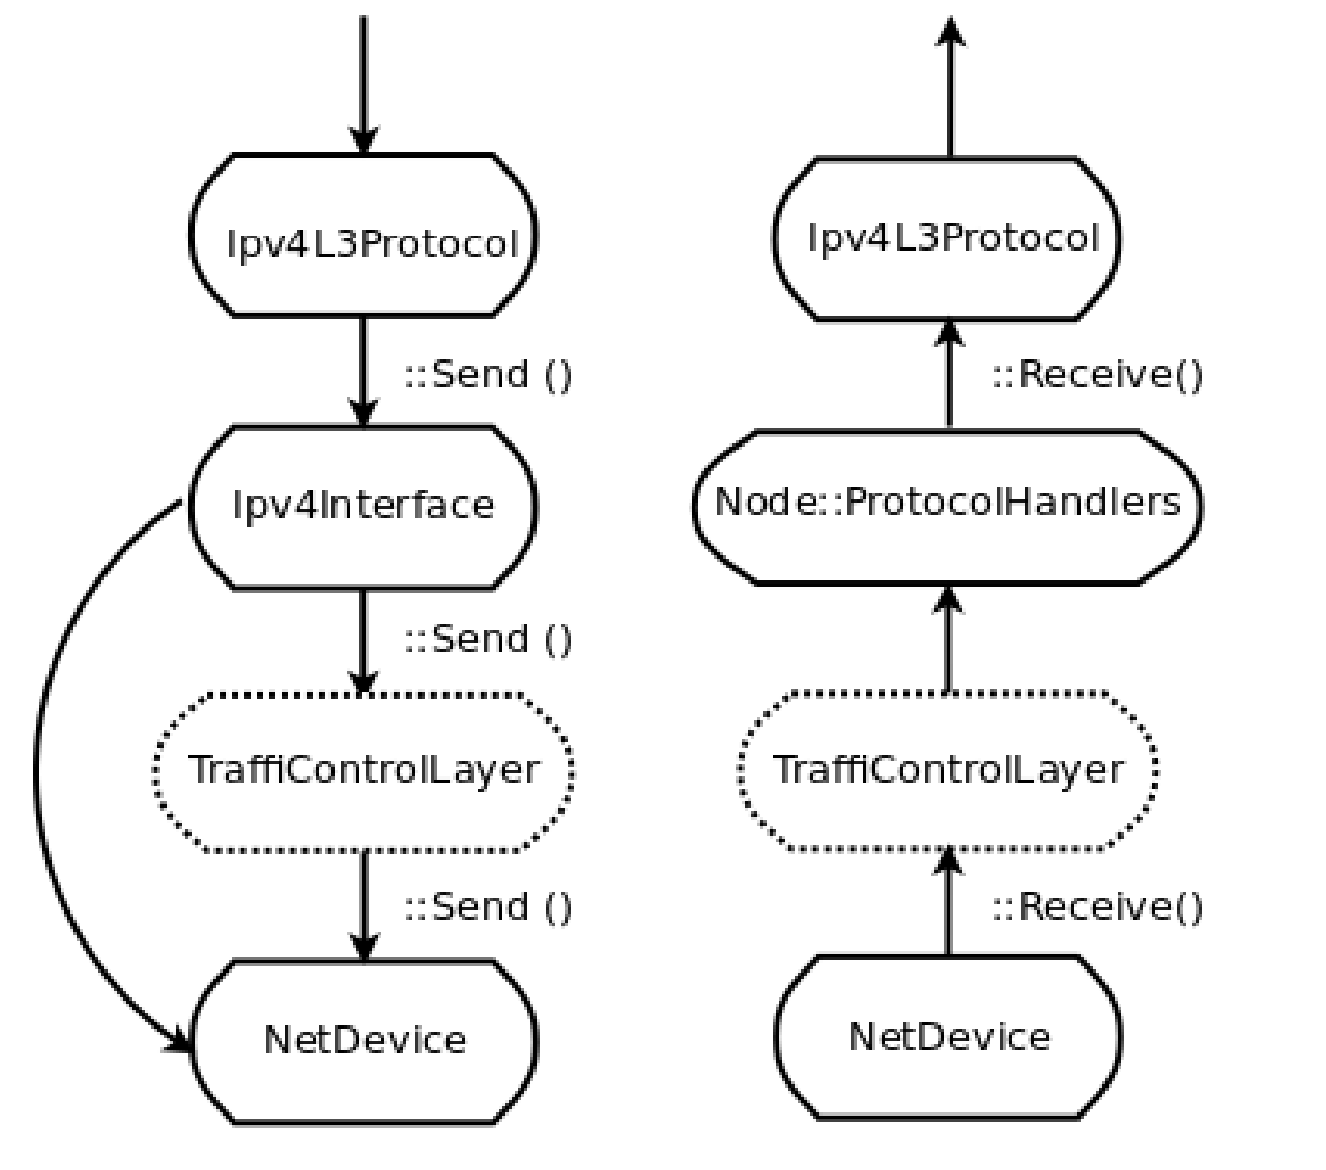
\includegraphics[height=150pt]{figs/ns3-queue.png}
\end{frame}


\begin{frame}{Summary}
Current ndnSIM consumer apps very limited! 

\begin{itemize}
\item [$\Rightarrow$] \textbf{Works much better now!}
\end{itemize}

\pause
Mechanisms:
\begin{enumerate}
\item Slow start + Congestion avoidance
\pause
\item Fast recovery + Conservative Window Adaptation
\pause
\item \textbf{Explicit Congestion Marks}
\pause
\item \textbf{CUBIC \textgreater\ AIMD}
\end{enumerate}


\end{frame}



%\begin{frame}{Experimental environment}
%
%Local topology:
%
%\begin{itemize}
%\item UDP Tunnels \& TCP Tunnels
%\item Ethernet \& WiFi
%\end{itemize}
%
%\end{frame}
%
%\begin{frame}{Results (WiFi):}
%
%\textbf{UDP (both links):}\\[.3em]
%\begin{tabular}{ l r l r }
%\toprule
%\textbf{Scenario} & \textbf{RTT}	& \textbf{Goodput} & \textbf{Retx} \\
%\midrule
%Without CC: & 60ms 	& 28.7 Mbps	 & 250 Retx \\
%With CC: & 6-9ms 		& 26.0 Mbps		 & 0 Retx \\
%\bottomrule
%\end{tabular}
%
%\pause
%\vspace*{1em}
%
%\textbf{TCP (both links):}\\[.3em]
%\begin{tabular}{ l r l r }
%\toprule
%\textbf{Scenario} & \textbf{RTT}	& \textbf{Goodput} & \textbf{Retx} \\
%\midrule
%Without CC: & 115ms 	& 37 Mbps	 & 320 Retx \\
%With CC: 		& 	7ms  	& 29 Mbps	 & 0 Retx \\
%\bottomrule
%\end{tabular}
%
%\vspace*{1em}
%
%\pause
%Ethernet: Cong. signals can even give you a \textbf{higher goodput!}
%
%\end{frame}
%
%
%\begin{frame}{Results (WiFi):}
%
%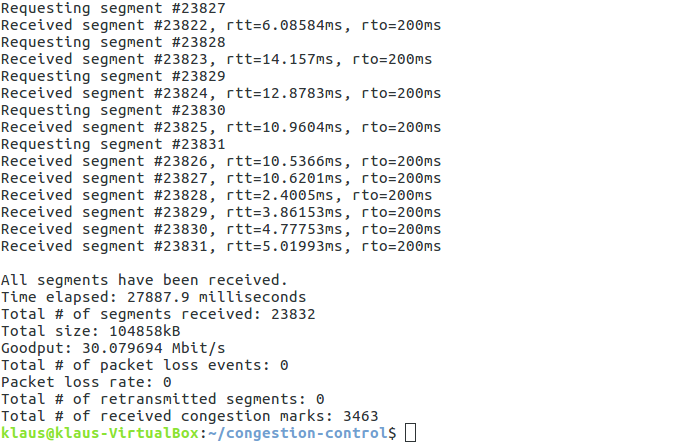
\includegraphics[width=\linewidth]{../results/screenshots.png}
%
%\end{frame}



%% Last slide
\begin{frame}
	\frametitle{The End}
	\vspace{2cm}
	{\huge Any Questions?
%		Thank you for
%		your attention!\\
%		\vspace*{2em}
	}
	\vspace{2.5cm}  
	\begin{flushright}  
		Klaus Schneider, Ashiqur Rahman, Chavoosh Ghasemi \\
%		 \footnotesize{
%%			\url{klaus@cs.arizona.edu} \\
%%			\url{https://www.cs.arizona.edu/~klaus/} %\\ 
%		}
	\end{flushright}
\end{frame}
